\section{Hand-made Data Structures}
\begin{frame}
  \begin{center}
    {\large Lecture 02 -- Data Structures\\Part IV -- Hand-made Data Structures}\\
  \end{center}
\end{frame}

\subsection{Motivation}
\begin{frame}
  \frametitle{Hand-making Data Structures}

  \begin{block}{}
    For certain problems, it is necessary to extend existing data structures;
  \end{block}

  \begin{itemize}
    \item Extensions of Arrays and Vectors for complex data;
    \bigskip

    \item New features for indexing and/or searching;
    \bigskip

    \item Express special relationship between data items (ex: graphs)
  \end{itemize}

  We will examine two data structures now: UFDS and Segment Tree
\end{frame}

\subsection{Union-Find}
\begin{frame}
  \frametitle{Union-Find Disjoint Set (UFDS)}
  \framesubtitle{Motivating Problem}

  \begin{block}{Network Connections -- UVA793}
    Imagine a network with $n$ computers, some are connected to others.
    \bigskip

    {\bf Input:} A series of ``commands''
    \begin{itemize}
    \item c i j -- New Info: Computer $i$ is connected to computer $j$
    \item q i j -- Query: Is computer $i$ connected to computer $j$?
    \end{itemize}

    \bigskip
    {\bf Output:} The number of ``q'' with answer yes, and the number
    of ``q'' with answer no.
  \end{block}
\end{frame}

\begin{frame}
  \frametitle{Union-Find Disjoint Set (UFDS)}
  \framesubtitle{Motivating Problem -- Naive answer}

  \begin{block}{Neighborhood Graph}
    \begin{itemize}
    \item Initialize an $n\times n$ matrix with zeros.
    \item For every ``c i j'' input, $N_{i,j}$ and $N_{j,i}$ becomes 1.
    \item For every ``q i j'', we perform a breadth first search on the graph.
    \end{itemize}
  \end{block}


  \bigskip

  How good is this solution?
  \begin{itemize}
  \item Cost to insert a new connection: $O(1)$
  \item Cost to check if ``q i j'': $O(V+E)$
  \end{itemize}

  \bigskip We can do better!
\end{frame}

\begin{frame}
  \frametitle{Union-Find Disjoint Set}

  \begin{center}
    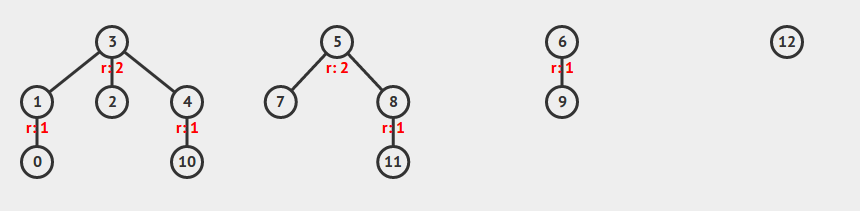
\includegraphics[width=.9\textwidth]{img/ufds1}
  \end{center}

  \begin{itemize}
  \item The UFDS keeps \structure{sets of items}, each is represented by a \structure{parent};
  \item When you join two sets \structure{You join their parents};
  \item When you test the parent of an item \structure{You flatten the tree};
  \item Test\_item and Join\_item are both O(1);\hfill \emph{(amortized)}
  \item Visualization: \url{https://visualgo.net/ja/ufds};
  \end{itemize}
\end{frame}

\begin{frame}[fragile]
  \frametitle{UFDS Implementation using Arrays}

  {\small
\begin{verbatim}
int p[MAX], r[MAX];
                             # which groups x belong to?
int find(int x) { return x == p[x] ? x : p[x]=find(p[x]); }

int join(int x, int y) {     # x and y are the same group
    x = find(x), y = find(y);
    if(x != y) {
        if(r[x] < r[y])     { p[x] = y; r[y] += r[x]; }
        else                { p[y] = x; r[x] += r[y]; }
        return 1;
    }
    return 0;
}

void init() { # Initialize each element as separate group
    for(int i = 0; i < MAX; i++)  { p[i] = i; r[i] = 1; }
}
\end{verbatim}
}

\end{frame}

\begin{frame}
  \frametitle{Union Find Disjoint Set}
  \framesubtitle{Problem II -- War}
  {\small
  \begin{block}{}
    From a set of 10k people, some are friends, other are enemies.
    \begin{itemize}
      \item If A,B are friends, and B,C are friends, then A,C are friends
      \item If A,B are friends, and B,C are enemies, then A,C are enemies
      \item If A,B are enemies, and B,C are enemies, then A,C are friends
    \end{itemize}

    {\bf Input:} A series of commands from the set below:
    \begin{itemize}
    \item SetFriends(i,j) \hspace{1.1cm} SetEnemies(i,j)
    \item TestFriends(i,j) \hspace{1cm} TestEnemies(i,j)
    \end{itemize}

    {\bf Output:}
    \begin{itemize}
    \item If a ``SetFriends'' or ``SetEnemies'' is impossible, output ``-1''
    \item For a ``TestFriends'', ``TestEnemies'', output 0 - false, 1 - true
    \end{itemize}
  \end{block}}

\end{frame}

\begin{frame}
  \frametitle{Union Find Disjoint Set}
  \framesubtitle{Problem II -- War}

  This problem is similar to ``Networking'', but now you need to keep track of {\bf TWO} relations: Friends and Enemies.\bigskip

  There are different ways to implement this:
  \begin{itemize}
    \item Create one UFDS for friends, and one UFDS for enemies?
    \item Add a ``friend/enemy'' flag for each person?
  \end{itemize}
  \bigskip

  What other ideas can you think? Which one is easy/hard to implement?
\end{frame}

\subsection{Segment Tree}
\begin{frame}[fragile]
  \frametitle{Range Maximum Query -- RMQ}

  Suppose you have an array of values:
\begin{verbatim}
Value: 18 17 13 19 15 11 20
Index:  0  1  2  3  4  5  6
\end{verbatim}

\bigskip

The \structure{Range Maximum Query} problem asks you to \structure{find
the index with the maximum value} between two indexes:

\begin{itemize}
  \item RMQ(0,0) = 0
  \item RMQ(0,6) = 6
  \item RMQ(1,4) = 3
\end{itemize}

\bigskip

\alert{Naive Method:} loop from $i$ to $j$, find maximum value. $O(nk)$ steps\\
\medskip

But what is the number of {\bf Values (n)} or {\bf Queries (k)} is too big?
\end{frame}

\begin{frame}
  \frametitle{Segment Tree}

  \begin{itemize}
    \item {\bf Basic idea}: Binary tree with the max index in of each subtree.
    \bigskip

    \item {\bf Operation Costs:}
    \begin{itemize}
      \item Creation of the tree: \structure{$O(n)$}
      \item Query of a segment: \structure{$O(\log n)$}
      \item Update of the tree: \structure{$O(\log n)$} \hfill \alert{Important Part}
    \end{itemize}
    \bigskip

    \item There are many implementations. We will show a vector based heap.
  \end{itemize}
\end{frame}

\begin{frame}
  \frametitle{Segment Tree}
  \begin{center}
    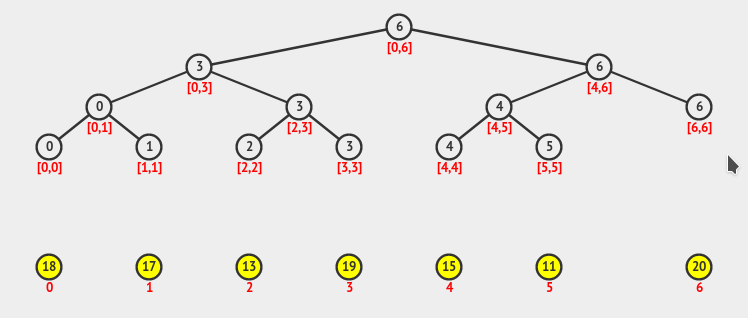
\includegraphics[width=1\textwidth]{img/segment_tree}
  \end{center}

  \bigskip

  Segment Tree animation at VISUALGO: \url{https://visualgo.net/en/segmenttree}
\end{frame}

\begin{frame}[fragile]
  \frametitle{Coding the Segment Tree}
  \framesubtitle{Tree Creation}
{\smaller
\begin{block}{}
\begin{verbatim}
typedef vector<int> vi; // Summarizing types that we use often.

class SegmentTree { // OOP implementation,
private: vi st, A;  // vi: typedef vector<int> vi;
  int n;
  int left (int p) { return  p<<1; }  // heap-like index;
  int right(int p) { return (p<<1) + 1; }

  void build(int p, int L, int R) {   // O(n log n)
    if (L == R)
      st[p] = L;                      // store the index
    else {                            // recursive build
      build(left(p) , L          , (L+R)/2);
      build(right(p), (L+R)/2 + 1, R      );
      int p1 = st[left(p)], p2 = st[right(p)];
      st[p] = (A[p1] <= A[p2]) ? p1 : p2;
  } }
\end{verbatim}
\end{block}}
\ppagenote{Segment Tree Code from \url{https://github.com/stevenhalim/cpbook-code}}

\end{frame}

\begin{frame}[fragile]
  \frametitle{Coding the Segment Tree}
  \framesubtitle{Query the Tree}
{\smaller
\begin{block}{rmq(1, 0, n-1, i, j) -- Query from i to j.}
\begin{verbatim}
int rmq(int p, int L, int R, int i, int j) // O(log n)
{
  if (i >  R || j <  L)
    return -1;    // outside query range
  if (L >= i && R <= j)
    return st[p]; // inside query range

  // compute the min position in the left and right part
  int p1 = rmq(left(p) , L        , (L+R)/2, i, j);
  int p2 = rmq(right(p), (L+R)/2+1, R      , i, j);

  if (p1 == -1) return p2;   // segment outside query
  if (p2 == -1) return p1;   // segment outside query
  return (A[p1] <= A[p2]) ? p1 : p2;
}
\end{verbatim}
\end{block}}
\end{frame}

\begin{frame}[fragile]
  \frametitle{Coding the Segment Tree}
  \framesubtitle{Update the Tree}

{\smaller
\begin{block}{update(1, 0, n-1, i, v) -- update index i to value v}
\begin{verbatim}
int update(int p, int L, int R, int idx, int new_value) {
  int i = idx, j = idx;    //for point update i = j = idx
  // if the curr interval does not intersect the update,
  if (i > R || j < L) return st[p];  //return node value!
  // if the current interval is in the update range,
  if (L == i && R == j) {
    A[i] = new_value;     // update the underlying array
    return st[p] = L;     // this index
  }
  // compute the min pos in L/R part of the interval
  int p1, p2;
  p1=update(left(p) , L        , (L+R)/2, idx, new_value);
  p2=update(right(p), (L+R)/2+1, R      , idx, new_value);
  // return the position where the overall minimum is
  return st[p] = (A[p1] <= A[p2]) ? p1 : p2;
}
\end{verbatim}
\end{block}}
\end{frame}
